\chapter{Formato Intel (Archivo .hex)}
\label{C:anexo_formato_intel}

El formato de archivo de objeto hexadecimal de Intel, el formato hexadecimal de Intel o Intellec Hex es un formato de archivo que transmite información binaria en forma de texto ASCII \cite{dot-hex-file}. Se usa comúnmente para programar microcontroladores, EPROM y otros tipos de dispositivos lógicos programables y emuladores de hardware. En una aplicación típica, un compilador o ensamblador convierte el código fuente de un programa (como en lenguaje C o ensamblador) en código de máquina y lo envía a un archivo \texttt{.hex}. Algunos también lo usan como un formato contenedor que contiene paquetes de datos de transmisión. Las extensiones de archivo comunes utilizadas para los archivos resultantes son \texttt{.hex} o \texttt{.H86}. Luego, un programador lee el archivo \texttt{.hex} para escribir el código máquina en una memoria o se transfiere al sistema de destino para su carga y ejecución.

\begin{figure}[ht!]
\centering
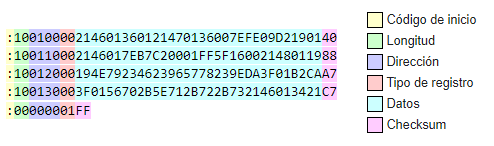
\includegraphics[width=0.7\textwidth]{./imagenes/hex-ejemplo.png}
\caption{ejemplo de archivo \texttt{.hex}}
\label{F:hex-ejemplo}
\end{figure}

\begin{description}
   \item[Código de inicio] El código de inicio utilizado es dos puntos ":"
   \item[Longitud del registro] Dos dígitos hexadecimales con la cantidad de bytes del campo de datos.
   \item[Dirección] Cuatro dígitos hexadecimales, con la dirección de inicio de los datos.
   \item[Tipo de registro] Dos dígitos hexadecimales, de 00 a 05, definen el tipo del campo de datos.
   \item[Datos] Duplas de dígitos hexadecimales que contienen los datos
   \item[Checksum] Dos dígitos hexadecimales con el complemento a dos de la suma de todos los campos anteriores, salvo el ":"
\end{description}

Hay seis tipos de registros, los mismos se describen a continuación:

\begin{description}
    \item[00] \underline{Datos}: La \textit{Longitud de registro} especifica el número de bytes de datos en el registro. El ejemplo tiene \colorbox{YellowGreen}{0B} (once) bytes de datos. La dirección inicial de 16 bits para los datos (en el ejemplo, en direcciones que comienzan en \colorbox{Periwinkle}{0010}) y los datos (\colorbox{SkyBlue}{61}, \colorbox{SkyBlue}{64}, \colorbox{SkyBlue}{64}, \colorbox{SkyBlue}{72}, \colorbox{SkyBlue}{65}, \colorbox{SkyBlue}{73}, \colorbox{SkyBlue}{73}, \colorbox{SkyBlue}{20}, \colorbox{SkyBlue}{67}, \colorbox{SkyBlue}{61}, \colorbox{SkyBlue}{70}).
    
    \underline{Ejemplo:} \colorbox{GreenYellow}{:}\colorbox{LimeGreen}{0B}\colorbox{Periwinkle}{0010}\colorbox{Peach}{00}\colorbox{SkyBlue}{6164647265737320676170}\colorbox{Lavender}{A7}
    
    \item[01] \underline{Fin de archivo}: Debe ocurrir exactamente una vez por archivo en el último registro del archivo. La Longitud siempre es \colorbox{YellowGreen}{00}, el campo de dirección suele ser \colorbox{Periwinkle}{0000} y se omite el campo de datos.
    
    \underline{Ejemplo:} \colorbox{GreenYellow}{:}\colorbox{LimeGreen}{00}\colorbox{Periwinkle}{0000}\colorbox{Peach}{01}\colorbox{Lavender}{FF}
    
    \item[02] \underline{Dirección Extendida de Segmento}: El Tipo de Registro siempre es \colorbox{Peach}{02}, el campo de dirección (normalmente \colorbox{Periwinkle}{0000}) se ignora y el campo de datos contiene una dirección base de segmento de 16~bits. Esto se multiplica por 16 y se suma a cada dirección de registro de datos subsiguiente para formar la dirección inicial de los datos. Esto permite direccionar hasta un mebibyte (1048576~bytes) de espacio de direcciones.

    \underline{Ejemplo:} \colorbox{GreenYellow}{:}\colorbox{LimeGreen}{02}\colorbox{Periwinkle}{0000}\colorbox{Peach}{02}\colorbox{SkyBlue}{1200}\colorbox{Lavender}{EA}
    
    \item[03] \underline{Dirección de Comienzo de Segmento}: Para procesadores 80x86, especifica la dirección de ejecución inicial. El Tipo de Registro siempre es \colorbox{Peach}{04}, el campo de dirección es \colorbox{Periwinkle}{0000} y los dos primeros bytes de datos son el valor CS, los dos últimos son el valor IP.
    
    
    \underline{Ejemplo:} \colorbox{GreenYellow}{:}\colorbox{LimeGreen}{04}\colorbox{Periwinkle}{0000}\colorbox{Peach}{03}\colorbox{SkyBlue}{00003800}\colorbox{Lavender}{C1}
    
    \item[04] \underline{Dirección Lineal Extendida}: Permite direccionamiento de 32~bits (hasta 4~GiB). La Longitud de bytes siempre es \colorbox{LimeGreen}{02} y el campo de dirección se ignora (normalmente \colorbox{Periwinkle}{0000}). Los dos bytes de datos especifican los 16 bits superiores de la dirección absoluta de 32~bits para todos los registros de tipo \colorbox{Peach}{00} posteriores; estos bits de dirección superiores se aplican hasta el siguiente registro \colorbox{Peach}{04}. La dirección absoluta para un registro de tipo \colorbox{Peach}{00} se forma combinando los 16~bits de dirección superiores del registro \colorbox{Peach}{04} más reciente con los 16~bits de dirección inferiores del registro \colorbox{Peach}{00}. Si un registro de tipo \colorbox{Peach}{00} no está precedido por ningún registro de tipo \colorbox{Peach}{04}, sus 16~bits de dirección superiores se establecen de forma predeterminada en \colorbox{Periwinkle}{0000}.
    
    \underline{Ejemplo:} \colorbox{GreenYellow}{:}\colorbox{LimeGreen}{02}\colorbox{Periwinkle}{0000}\colorbox{Peach}{04}\colorbox{SkyBlue}{FFFF}\colorbox{Lavender}{FC}
    
    \item[05] \underline{Comienzo de Dirección Lineal}: La Longitud de bytes siempre es \colorbox{LimeGreen}{04}, el campo de dirección es \colorbox{Periwinkle}{0000}. Los cuatro bytes de datos representan un valor de dirección de 32~bits. En el caso de las CPU que lo soportan, esta dirección de 32~bits es la dirección de ejecución inicial).
    
    \underline{Ejemplo:} \colorbox{GreenYellow}{:}\colorbox{LimeGreen}{04}\colorbox{Periwinkle}{0000}\colorbox{Peach}{05}\colorbox{SkyBlue}{000000CD}\colorbox{Lavender}{2A}
    
\end{description}